\section{Case Studies}\label{sec:casestudy}


To demonstrate the utility of our modular parsing approach, we
implemented parsers of the first 18 calculi from book \textit{Types
  and Programming Languages} (TAPL) \cite{pierce2002types}. TAPL introduces several
calculi from simple to complex, by gradually adding new features to
syntax. We compared our implementation with a non-modular implementation
we found online, which is also written in Scala and uses the same Packrat parsing library.
We counted source lines of code (SLOC) and measured execution time for both implementations.
Our implementation saves almost 70\% code comparing with that non-modular one.

\huang{done}\bruno{mention that you compare against an existing non-modular implementation.}

\subsection{Implementation}

The calculi in the TAPL book are suitable for our case study for mainly two reasons.
Firstly, the calculi are arguably capture many of the language features
required in realistic programming languages. Secondly, the evolution of
calculi in the book reveals the advantages of modular representation
of abstract syntax and modular parsing, which is the key functionality
of our approach. By extracting common components from those calculi
and reusing them, we obtain considerably code reuse with reasonable performance penalty, as shown later.

\paragraph{Extracting Language Components}
Using the modular parsing techniques discussed before, we extract
reusable components from syntax of all the calculi. Each
component, which may contain several syntactical structures,
represents a certain feature of the language. For
example, the \lstinline{VarApp} component below represents variables and
function applications.

\huang{todo: move the code, rename PackratParser}
\begin{lstlisting}
object VarApp {
  trait Alg[E] {
    def TmVar(x: String): E
    def TmApp(e1: E, e2: E): E
  }
  trait Print extends Alg[String] {
    def TmVar(x: String): String = x
    def TmApp(e1: String, e2: String): String = "[" + e1 + " " + e2 + "]"
  }
  trait Parser[E] extends EParser[E] {
    lexical.delimiters += ("(", ")")
    val alg: Alg[E]
    val pVarAppE: PackratParser[E] = {
      lcid ^^ alg.TmVar |||
        pE ~ pE ^^ { case e1 ~ e2 => alg.TmApp(e1, e2) } |||
        "(" ~> pE <~ ")"
    }
  }
}
\end{lstlisting}

In our case study, each component is represented by a Scala object which has three parts.
\lstinline{Alg} is an object algebra interface for the abstract syntax.
\lstinline{Print} is an object algebra implements that interface
\lstinline{Alg}, for the pretty printing operation. They are standard object algebra operations.
\lstinline{Parser} is the modular parser for this piece of syntax.

We have some naming conventions in our code, \lstinline{E} represents
expressions, \lstinline{T} represents types and \lstinline{K}
represents kinds. They are the three sorts of syntax in our case study.
In this particular component \lstinline{VarApp} we only have expressions.

Similar as before, each parser carries lexical information, an object algebra field, and
parsing functions. We have some helper traits for convenience, such as \inlinecode{EParser}
containing \inlinecode{pE} for parsing expressions.

\begin{lstlisting}
trait EParser[E] {
  val pE: PackratParser[E]
}
\end{lstlisting}

\paragraph{Composing Language Components}
Each calculus could be composed directly from components and other
calculi as needed. For example, the calculus \lstinline{Untyped} in our case study,
representing the famous untyped lambda calculus, is constructed from components \lstinline{VarApp}
and untyped lambda abstraction \lstinline{UntypedAbs}.

\begin{lstlisting}
object UntypedAbs {
  trait Alg[E] {
    def TmAbs(x: String, e: E): E
  }
  trait Print extends Alg[String] {
    def TmAbs(x: String, e: String): String = "\\" + x + "." + e
  }
  trait Parser[E] extends EParser[E] {
    lexical.delimiters += ("\\", ".", "(", ")")
    val alg: Alg[E]
    val pUntypedAbsE: PackratParser[E] =
      ("\\" ~> lcid) ~ ("." ~> pE) ^^ { case x ~ e0 => alg.TmAbs(x, e0) } |||
      "(" ~> pE <~ ")"
  }
}

object Untyped {
  trait Alg[E] extends UntypedAbs.Alg[E] with VarApp.Alg[E]
  trait Print extends Alg[String] with UntypedAbs.Print with VarApp.Print
  trait Parser[E] extends UntypedAbs.Parser[E] with VarApp.Parser[E] {
    override val alg: Alg[E]
    val pUntypedE: PackratParser[E] = pUntypedAbsE ||| pVarAppE
    override val pE: PackratParser[E] = pUntypedE
  }
}
\end{lstlisting}

When composing the calculus from components, all the traits can be
easily combined by Scala's \inlinecode{extends...with} keywords.
In \lstinline{Parser}, we need to override the object algebra interface and
parsing functions accordingly.

\paragraph{Demo code}
We have demo code for every calculus in order to test and evaluate our implementation.
We feed the pretty printing algebra to the parser and print out the result.
The parsing result can be changed as long as the concrete algebra is available.

\begin{lstlisting}
object TestUntyped {
  def work[E](inp: String)(a: Untyped.Alg[E]): E = {
    val lang = new Untyped.Parser[E] {
      override val alg: Untyped.Alg[E] = a
    }
    parse(lang.pE)(inp)
  }
  def parseAndPrint(inp: String): Unit = println(work(inp)(new Untyped.Print {}))
  def main(args: Array[String]): Unit = {
    parseAndPrint("(\\x.x) (\\y.y)")
  }
}
\end{lstlisting}

\paragraph{Dependency Overview}
Figure \ref{fig:dependency} shows the
dependency of all the components and calculi in our case study. Gray
boxes are calculi and white boxes are components. An arrow starting
from box A to box B denotes that B includes and thus reuses A.

\begin{figure}
    \centering
    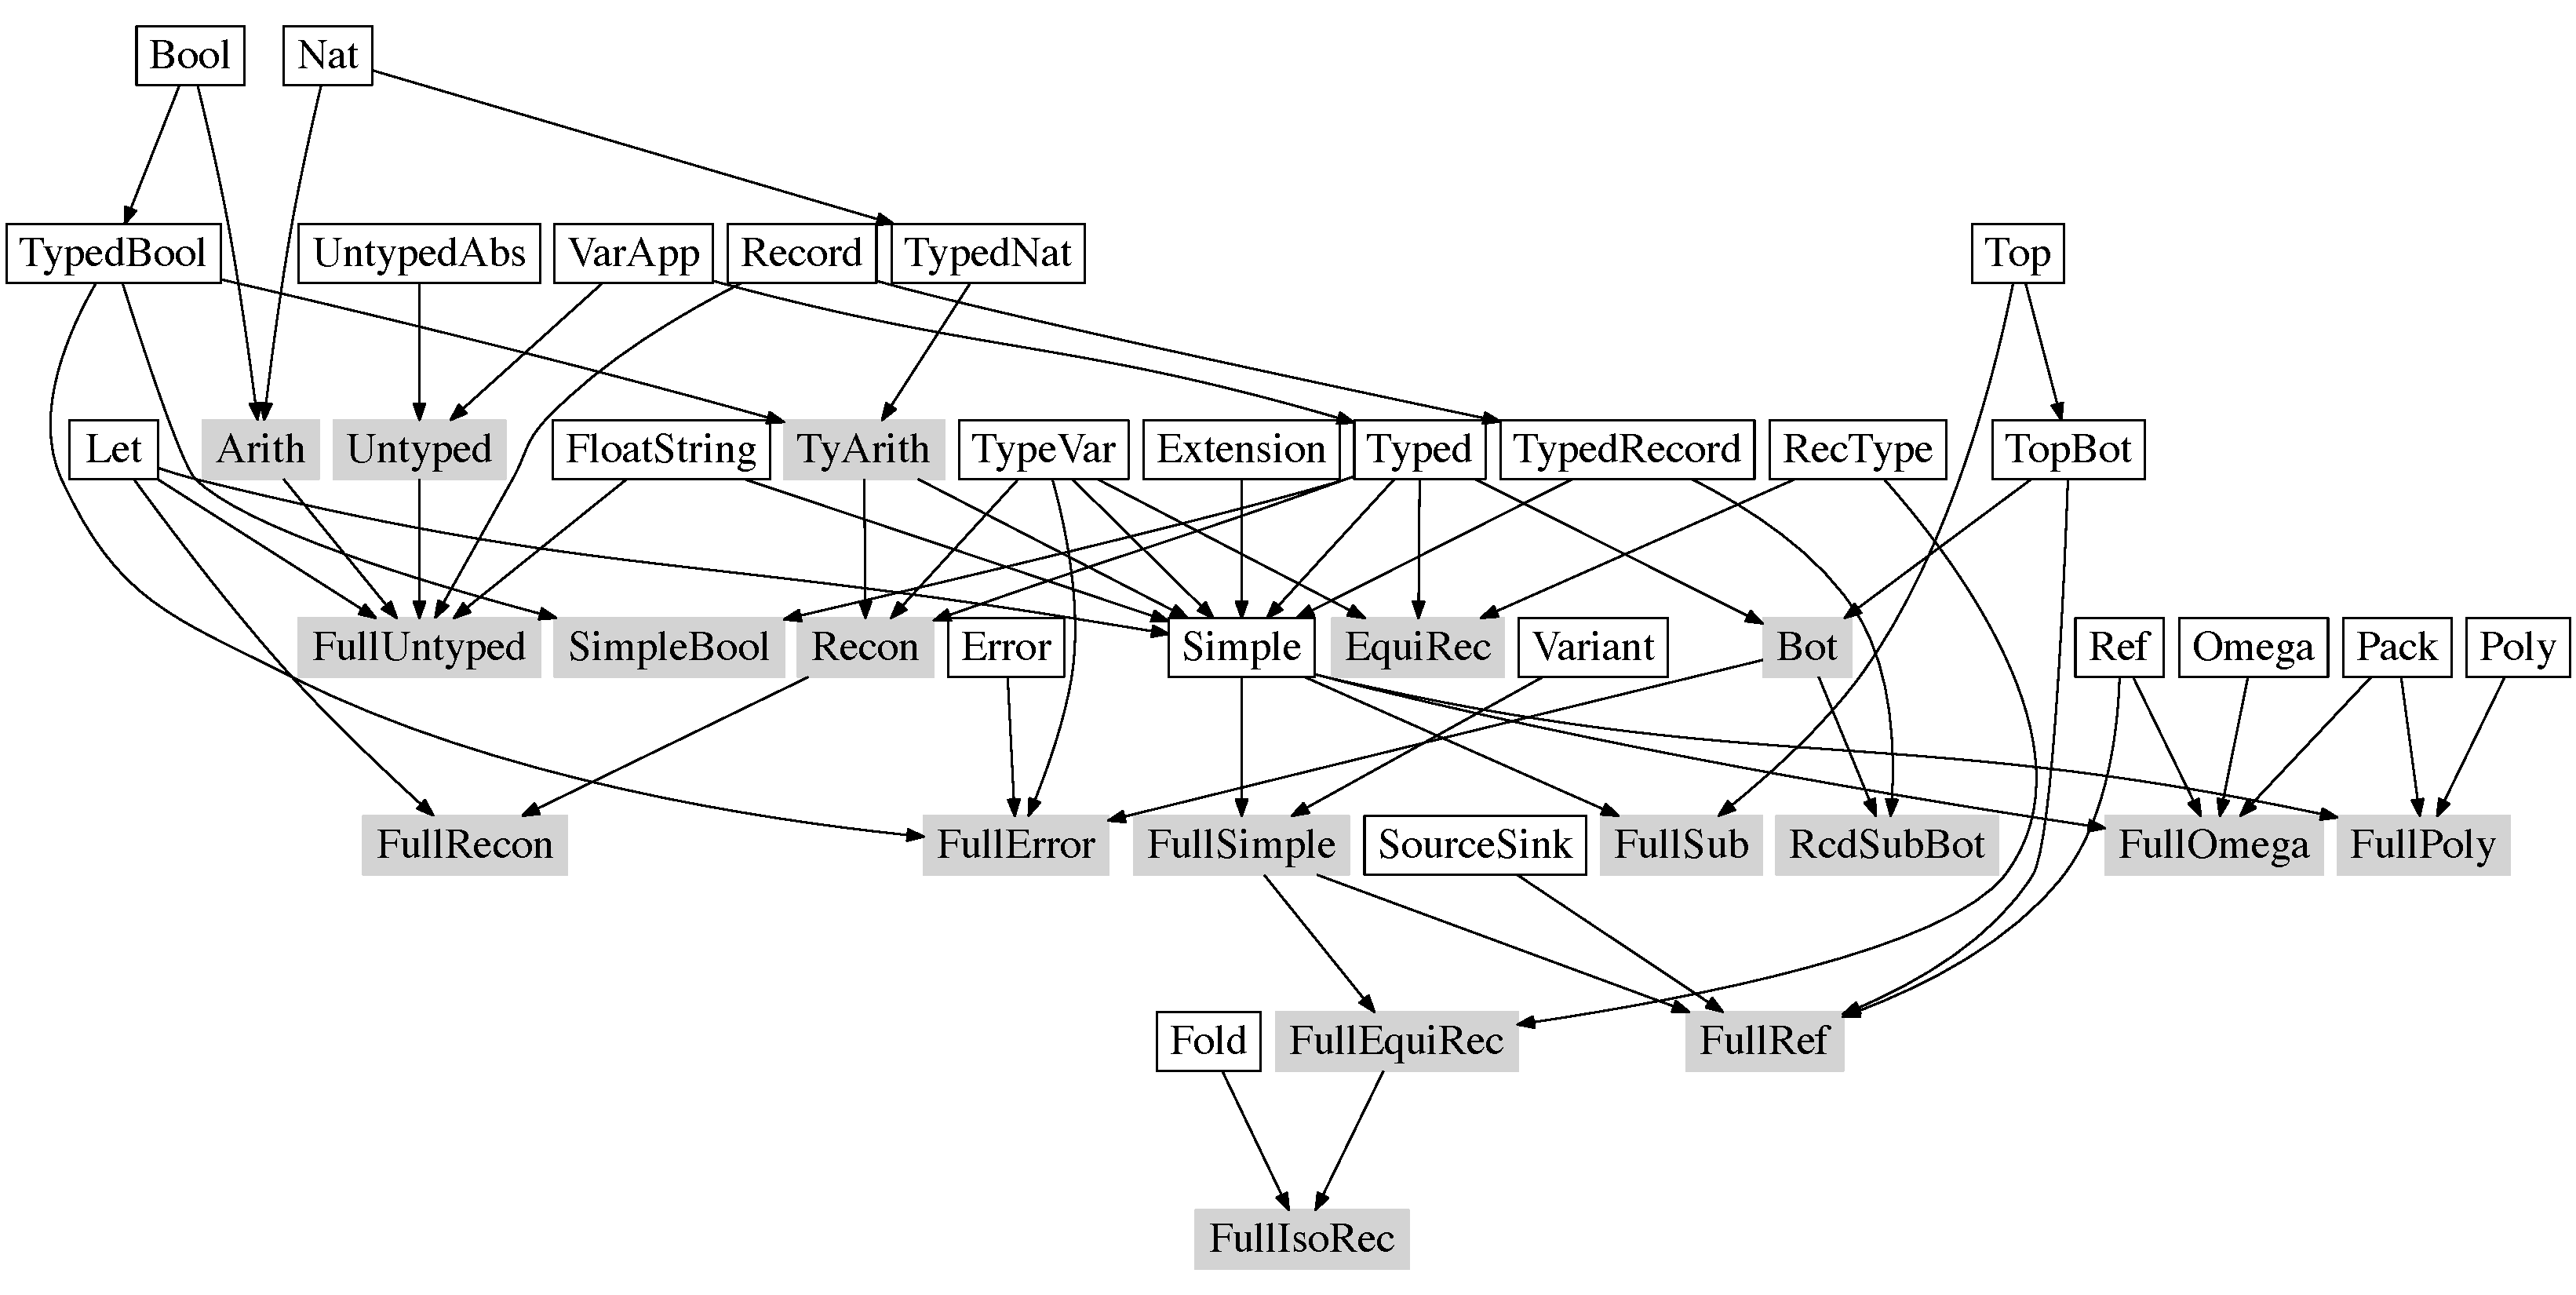
\includegraphics[width=\textwidth]{resources/depGraph.pdf}
    \caption{Dependency graph of all calculi and components}
    \label{fig:dependency}
\end{figure}

As shown in the graph, some components such as \lstinline{VarApp} are
created from scratch, while others such as \lstinline{Typed} are
extended from existing components. Since calculi and components have the similar signature, each calculus
can also be extended and reused directly. For example, calculus \lstinline{FullRef} extends from
calculus \lstinline{FullSimple}.

Using our modular parsing approach, it is convenient to extract language
features as components and reuse them. From the dependency graph, we know
that common components such as \lstinline{VarApp} are reused in
lots of calculi. Such reuse could shorten the code considerably. We
will show this advantage and exam the possible performance penalty in
a quantitative way in the next subsection.

\subsection{Comparison}\label{subsec:cs-comparison}

We compared our implementation of the parsers with an implementation
by Ilya Klyuchnikov, available online\footnote{https://github.com/ilya-klyuchnikov/tapl-scala/}.
Ilya's implementation is suitable for comparison, because it is also
written in Scala using the same parser combinator library.
Furthermore, it includes parsers of all the 18 calculi we have, but
written in a non-modular way. Thus it is not able to reuse existing
code when those calculi share common features.

The comparison is made from two aspects. First, we want to discover
the amount of code reuse using our modular parsing approach.
For this propose, we measured source lines of code (SLOC) of two implementations.
Second, we are interested to assess the performance penalty caused by modularity.
Thus we compared the execution time of parsing random expressions between two implementations.

\paragraph{Standard of Comparison}
In the SLOC comparison, all blank lines and comment lines are excluded,
and we formatted the code of both implementations to guarantee that
the length of each line does not exceed 120 characters. Furthermore,
because Ilya's implementation has extra code such as semantics,
we removed all irrelevant code and only keep abstract
syntax definition, parser and pretty printer for each calculus, to
ensure a fair comparison.

For the comparison of execution time, we built a generator to randomly
generate valid expressions of each calculus, according to the syntax. These expressions are
written to test files, one file per calculus. Each test file consists of 500
expressions randomly generated, and the size of test files varies from 20KB to 100KB.
Then we run the corresponding parser to parse the file and the pretty printer to print the result.
The average execution time of 5 runs excluding reading input file was calculated, in milliseconds.

\huang{done}\bruno{say something about what those expressions are, size, and how they were generated.}

\begin{table}
    \centering
    \begin{tabular}{|l|r|r|r|r|r|r|}
      \hline
        \multirow{2}{*}{\bfseries Calculus Name} & \multicolumn{3}{ c| }{\bfseries SLOC} & \multicolumn{3}{ c| }{\bfseries Time (ms)} \\ \cline{2-7}
        \multicolumn{1}{|c|}{} & \bfseries Ilya's & \bfseries Ours & \bfseries (+/-)\% & \bfseries Ilya's & \bfseries Ours & \bfseries (+/-)\% \\
      \hline
      \begin{tabular}{|c|c|c|}
  \hline
  t1 & t2 & t3 \\
  y1 & val1 & val4 \\
  y2 & val2 & val3 \\
  \hline
\end{tabular}

      \hline
    \end{tabular}
    \caption{Comparison of SLOC and execution time}
    \label{tab:comparison}
\end{table}

\paragraph{Comparison Results}
Table \ref{tab:comparison} shows results of the comparison.
The overall result is that 69.2\% of code is reduced using our
library, and our implementation is 42.7\% slower.

The good SLOC result is because of that the code of common language features
such as variables, lambda abstractions, etc., are reused lots of times in
the whole case study. We can see that in the first two calculi
\lstinline{Arith} and \lstinline{Untyped} we are not better than Ilya's
implementation, because in such two cases we do not reuse any existing
components. However in the following 16 calculi, we can reuse
language components, resulting considerably code reduction. In particular,
the calculi \inlinecode{EquiRec}, \inlinecode{Recon} and some others are only 22 lines
in our implementation, because we only compose existing codes in such cases.

To discover the reasons of slower execution time, we made some more experiments
on two possible factors which could affect the performance.
They are object algebra and the longest match alternative combinator.
We use object algebra for ASTs and the longest match alternative combinator \inlinecode{|||} for parsing,
while Ilya's implementation uses case class and the ordinary alternative combinator.

We implemented two more versions. One is a modified version of our implementation,
with object algebra replaced by case class for the ASTs.
The other is a modified version of Ilya's implementation, using the longest match
alternative combinator instead of the ordinary one.

\huang{done}\bruno{A table showing a summary of results is missing here. We discussed this before.}

\begin{table}
    \centering
    \begin{tabular}{|l|r|r|r|r|r|r|r|}
      \hline
        \multirow{2}{*}{\bfseries Calculus Name} & \bfseries Ilya's & \multicolumn{2}{ c| }{\bfseries Ours} & \multicolumn{2}{ c| }{\bfseries Ilya's with \inlinecode{|||}} & \multicolumn{2}{ c| }{\bfseries Ours with class} \\ \cline{3-8}
        \multicolumn{1}{|c|}{} & \multicolumn{1}{c|}{\bfseries Time} & \bfseries Time & \bfseries (+/-)\% & \bfseries Time & \bfseries (+/-)\% & \bfseries Time & \bfseries (+/-)\% \\
      \hline
        Arith & 741 & 913 & +23.2 & 793 & +7.0 & 932 & +25.8 \\
        Untyped & 770 & 1018 & +32.2 & 821 & +6.6 & 1007 & +30.8 \\
      \hline
        \multicolumn{1}{|c|}{\dots} & \multicolumn{7}{c|}{\dots} \\
      \hline
        FullRecon & 1094 & 1645 & +50.4 & 1161 & +6.1 & 1652 & +51.0 \\
        FullPoly & 1398 & 2086 & +49.2 & 1511 & +8.1 & 2019 & +44.4 \\
        FullOmega & 1451 & 2352 & +62.1 & 1582 & +9.0 & 2308 & +59.1 \\
      \hline
        Total & 21746 & 31024 & +42.7 & 23260 & +7.0 & 30795 & +41.6 \\
      \hline
    \end{tabular}
    \caption{Execution time of four versions}
    \label{tab:ext-comparison}
\end{table}

Table \ref{tab:ext-comparison} shows part of the comparison results of these four versions,
full table is available online []. It suggests that the difference of running time between
using object algebra and class is little, roughly 1\%.
The usage of longest match combinator slows the performance by 7\%. The main reason of slower
execution time may be the overall structure of the modular parsing approach, because we indeed have
more intermediate function calls and method overriding. However, it is worth metioning that
because of the memoization technique of Packrat parsers, we are only constant times
slower, the algorithmic complexity is still the same.

